% rubber: set program xelatex
%!TEX root=thesis.tex
\RequirePackage[]{silence}
\RequirePackage[l2tabu, orthodox]{nag}

\documentclass[fontsize=11pt,paper=a4,twoside,openright]{scrreprt}

\usepackage[automark]{scrpage2}% mit automatischen Kolumnentiteln
\clearscrheadings% Seitenstil scrheadings leeren
\ohead{\headmark}% Kolumnentitel im Kopf außen
\cfoot{\pagemark}% Paginierung im Fuß zentriert
\pagestyle{scrheadings}
\usepackage[usenames,dvipsnames]{xcolor}
\usepackage{polyglossia}
\usepackage{fontspec}
\usepackage{nomencl}
\usepackage{eqlist}
\usepackage{tabularx}
\usepackage{caption}
\usepackage[numbers,square]{natbib}
\usepackage{subcaption}
\usepackage{multicol}
\usepackage{graphicx}
\usepackage[hyperfootnotes=false]{hyperref}
\usepackage{shadethm}
\usepackage{parskip}
\usepackage{subcaption}
\usepackage{float}
\usepackage{wrapfig}
\usepackage{listings}

\defaultfontfeatures{Mapping=tex-text}
\defaultfontfeatures{Ligatures={NoRequired, NoCommon, NoContextual, TeX}}

\usepackage{glossaries}
\usepackage[left=30mm,right=20mm,top=25mm,bottom=25mm]{geometry}

% Doppelter Zeilenabstand:
\usepackage{setspace}
\usepackage{amsmath}

\setboolean{@twoside}{false}
%!TEX root=mt.tex
\graphicspath{{./img/}}

%\SetProtrusion{encoding={*},family={bch},series={*},size={6,7}}
%              {1={ ,750},2={ ,500},3={ ,500},4={ ,500},5={ ,500},
%               6={ ,500},7={ ,600},8={ ,500},9={ ,500},0={ ,500}}
%\SetExtraKerning[unit=space]
%   {encoding={*}, family={qhv}, series={b}, size={large,Large}}
%   {1={-200,-200}, 
%    \textendash={400,400}}

\setdefaultlanguage{german}
\bibliographystyle{natdin}
%\bibliographystyle{alphadin}

%\deftranslation[to=german]{Acronyms}{Abkürzungsverzeichnis}
%\deftranslation[to=german]{Contents}{Inhaltsverzeichnis}
%\deftranslation[to=ngerman]{Acronyms}{Abkürzungsverzeichnis}

\clubpenalty=10000
\widowpenalty=10000
\displaywidowpenalty=10000

%\setmainfont{Adobe Garamond Pro} % Main document font
%\setsansfont{Gill Sans} % Used in the from address line above the to address
%\setmainfont[Ligatures={NoRequired,NoCommon,NoContextual}]{}

\newshadetheorem{definition_}{Definition}
\newenvironment{definition}[1][]{%
  \definecolor{shadethmcolor}{rgb}{.9,.9,.9}%
  \definecolor{shaderulecolor}{rgb}{0.0,0.0,0.0}%
  \setlength{\shadeboxrule}{1pt}%
  \begin{definition_}[#1]%
}{\end{definition_}}

\let\description=\eqlist
\let\enddescription=\endeqlist
\let\eqlistlabel\descriptionlabel


\makeglossary
\newcounter{alteSeitenzahl}

\setlength{\parindent}{0cm}

\setcounter{tocdepth}{2} 
\setcounter{secnumdepth}{2}
\begin{document}
\renewcommand{\refname}{Literaturverzeichnis}

\pagenumbering{Roman}
%!TEX root=mt.tex
%\newacronym{SDK}{SDK}{Ein Softwarepaket für die Entwicklung von Software auf Basis einer bestimmten Zielplattform}
\newglossaryentry{SDK}{name=Software Development Kit,
description={Ein Softwarepaket für die Entwicklung von Software auf Basis einer bestimmten Zielplattform}}
\newglossaryentry{AGV}{name=Automated Guided Vehicle,
description={Ein sich selbst steuerndes Fahrzeug, welches einer bestimmten optischen oder magnetischen Markierung auf dem Boden folgt}}
\newglossaryentry{ROS}{name=Robot Operating System,
description={Ein unabhängiges Roboterbetriebssystem, welches 2007 an der Universität Stanford ins Leben gerufen wurde}}
%!TEX root=mt.tex
\author{Ullrich}
\begin{titlepage}
\begin{center}
\newcommand{\HRule}{\rule{\linewidth}{0.5mm}}

\textsc{\large Technische Hochschule N\"urnberg Georg-Simon-Ohm}\\[0.3cm]

\textsc{\normalsize Fakult\"at Informatik}\\[1.0cm]

\textsc{\large Wintersemester 2012/13}\\[1.0cm]

% Title
\setlength{\baselineskip}{2.0\baselineskip}


\HRule\\[0.5cm]
{\Large \bfseries Evaluierung und Implementierung eines Konzeptes für die autonome Orientierung eines humanoiden Roboters\\[0.5cm]
\large \bfseries anhand potentieller Warnzeichen oder Gefahrensituationen\\[0.2cm]}

\HRule\\[1.5cm]
        %\texttt{}\\
        %\texttt{UllrichCh35492@ohm-hochschule.de}\\
\Large{Masterarbeit}\\        
{\href{mailto:UllrichCh35492@ohm-hochschule.de}{\Large Christian~A.~Ullrich}}\\
{\href{mailto:UllrichCh35492@ohm-hochschule.de}{\large UllrichCh35492@ohm-hochschule.de}} \\[0.4cm]

\begin{minipage}{0.6\textwidth}
\begin{center}
\textsc{\large Erstkorrektor}\\[0.3cm]
{\large
\href{mailto:Florian.Gallwitz@ohm-hochschule.de}{Prof.~Dr.-Ing.~Florian~Gallwitz}} \\[0.4cm]
\textsc{\large Zweitkorrektor}\\[0.3cm]
{\large
\href{mailto:Rainer.Rieckeheer@ohm-hochschule.de}{Prof.~Dr.~Rainer~Rieckeheer}} \\

%\textsc{\small Georg-Simon-Ohm Hochschule N\"urnberg} \\[0.3cm]
\end{center}
\end{minipage}

\vfill

% Bottom of the page
{
\textsc{\small Technische Hochschule N\"urnberg Georg-Simon-Ohm} \\[0.3cm]
\large 15. April 2013}


\end{center}
\end{titlepage}

\newpage
\section*{}

%!TEX root=mt.tex
\section*{Eigenständigkeitserklärung}
Ich versichere hiermit, dass ich die vorliegende Abschlussarbeit selbstständig verfasst, nicht anderweitig für Prüfungszwecke vorgelegt und keine anderen als die angegebenen Hilfsmittel und Quellen benutzt habe.
Die Stellen, die anderen Werken dem Wortlaut oder dem Sinn nach entnommen wurden, habe ich in jedem einzelnen Fall durch die Angabe der Quelle, auch der benutzten Sekundärliteratur, als Entlehnung kenntlich gemacht.
	
\vspace{15cm}
\begin{tabularx}{\textwidth}[b]{p{9cm} X p{5cm}} \cline{1-1} \cline{3-3}
Christian Ullrich & & Ort, Datum\\
\end{tabularx}
\newpage

\newpage
\section*{}

\setcapindent{0em}
\raggedbottom
\chapter*{Vorwort}
\label{sec:Vorwort}

Diese Arbeit befasst sich mit einer Studie im Bereich der humanoiden Robotertechnologie. Es wird ein Konzept und eine prototypische Implementierung entworfen um einen Roboter der NAO-Serie durch eigenständige Analyse der Umwelt zu steuern und ihn dabei autonom nach möglichen Gefahrenquellen -- wie etwa Schildern oder Warnzeichen -- suchen zu lassen.

Hierbei wird vor allem auf die verschiedenen komplexen Teilaspekte einer solchen Problemstellung eingegangen.
So spielen unter anderem Inhalte aus der Optik, Kinetik als auch der menschlich-maschinellen Interaktion eine wesentliche Rolle in einem derartigen Konzept.
Die Konstruktion eines theoretischen Modells wird zunächst dabei helfen, potentielle Probleme aus den genannten Bereichen zu identifizieren und eine grundlegende Struktur für deren Lösung und Implementierung zu schaffen.
Es werden auch mögliche technische Grenzen analysiert.

Darüber hinaus wird eine anschließende Evaluation des \gls{SDK} des NAO-Roboters aufzeigen, inwieweit sich der gefundene Lösungsansatz in diesem reflektiert.
Es wird sich zeigen, ob gegebenenfalls weitere Software benötigt wird.

Eine prototypische Implementierung des Konzeptes wird dessen Umsetzbarkeit an einem echten Roboter testen.
Dabei wird von mehreren realistischen Szenarien ausgegangen, mit denen das System konfrontiert wird.

Das Ziel dieser Arbeit ist es, neben einem funktional korrekten Konzept bzw. der prototypischen Implementierung auch die Komplexität des Modellierungsprozesses eines derartigen Projektes herauszuarbeiten und aufzuzeigen.
Weiterhin soll die Frage beantwortet werden, inwieweit die Ergebnisse in den Rahmen bisheriger Theorien in der Robotik eingebettet werden können.

%Ein wesentlicher Anstoß für die Bearbeitung dieses Themas begründet sich in der persönlichen Motivation des Autors.
%Dieser hat sich im Laufe seines Studiums mit verschiedenen Themen befasst, welche immer eine gewisse Teilmenge der zu bearbeitenden Problemstellung beinhalteten.
%Die Idee an einem humanioden Roboter zu arbeiten, soll die angesammelten Kenntnisse im Bereich der Grafikverarbeitung, der Entwicklung auf mobilen Plattformen sowie der Etablierung neuartiger Bedienkonzepte vertiefen und festigen.

Als Vorwissen dienen Lerninhalte sowohl aus dem Bachelor- als auch dem Masterstudiengang Informatik.
Insbesondere wird auf Konzepte der Fächer Grundlagen multimedialer Systeme, Digitale Bildverarbeitung und Mustererkennung zurückgegriffen.
Darüber hinaus sind selbstverständlich die allgemein gültigen Grundlagen aus den Kursen Programmieren 1 und 2, Softwarearchitektur und Software Engineering für diese Arbeit maßgebliche Voraussetzungen.
Der Besitz von Kenntnissen über die Kreation von und dem Umgang mit humanoiden Robotersystemen ist für den Leser hilfreich, aber nicht zwingend erforderlich.

%Related Work, was studiert wurde evtl hier mit rein.

Alle in dieser Arbeit verwendeten Tabellen, Abbildungen, Codelistings und Abkürzungen sind in individuellen Verzeichnissen am Ende der Arbeit zur besseren Übersicht aufgelistet.
Begriffsdefinitionen und Anmerkungen sind -- soweit notwendig -- in den Fußnoten angegeben.
Wörtliche Zitate werden durch Anführungszeichen, Kursivschrift und einer Fußnote mit Quellenangabe kenntlich gemacht.
Sinngemäß übertragene Inhalte -- wie beispielsweise Abbildungen oder Denkansätze -- sind ebenfalls mit Fußnoten und Quellenangaben gekennzeichnet.

In dieser Arbeit genannte Personen bzw. Typen (z.B.\ der Leser) sind zumeist im generischen Maskulinum gehalten.
Dies soll keine sprachliche Diskriminierung, sondern lediglich einem vereinfachten Sprachverständnis dienen.

Die gesamte in der Arbeit verwendete Literatur, Dokumentation und Referenzwerke sind in einem entsprechenden Verzeichnis am Ende dieser Arbeit angegeben.

This is a small text. a very small test.

\clearpage

\newpage
\section*{}

\chapter*{Danksagung}
Der Autor bedankt sich bei den Supportmitarbeitern von Aldebaran Labs., Inc. für die Antwort auf technische Fragen, der Technischen Hochschule Nürnberg Georg-Simon-Ohm, für die Bereitstellung des Nao-Roboters und den Professoren Prof.\ Dr.\ Ing.\ Florian Gallwitz und Prof.\ Dr.\ Rainer Rieckeheer für die fachliche Betreuung während der Bearbeitungszeit.
\clearpage

\newpage
\section*{}

\setboolean{@twoside}{true} 
\singlespacing
\tableofcontents

\chapter{Einleitung}
\label{sec:Einleitung}
\setcounter{alteSeitenzahl}{\value{page}}
\pagenumbering{arabic}
\begin{wrapfigure}{r}{0.30\textwidth}
\vspace{-12pt}
  \centering
  \fbox{
    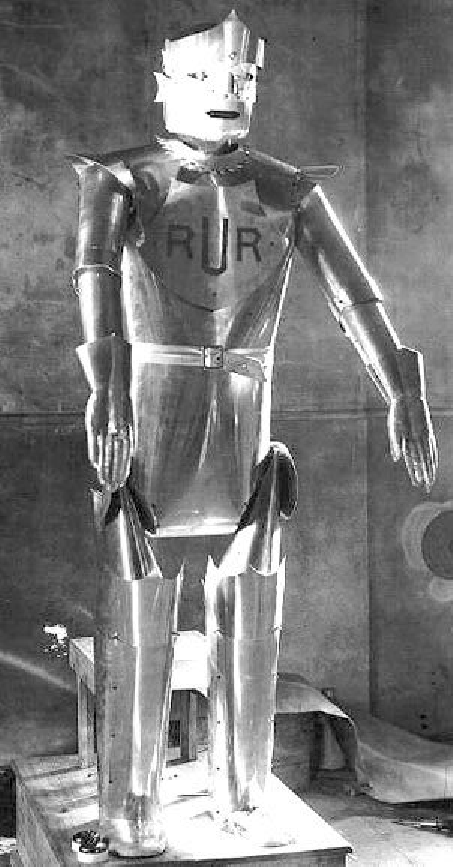
\includegraphics[width=0.225\textwidth]{rur_robot}
  }
  \caption[Roboter aus R.U.R.]{Roboter aus R.U.R.\protect \footnotemark}
\vspace{-10pt}
  \label{fig:Roboter aus R.U.R.}
\end{wrapfigure}
\footnotetext{Abbildung aus \cite{RoboHistoryHP}, Abschnitt What is a robot?}
Seit der tschechische Schriftsteller Karel Čapek mit seinem Theaterstück Rossums Universal-Robots im Jahre 1920 den heutzutage viel genutzten Terminus „Roboter“ prägte, sind zunehmend immer mehr Menschen an deren Technologie und Fähigkeiten interessiert.
Kein Wunder, versprechen doch diese seit der Verbreitung des Personal Computer in den späten siebziger Jahren der nächste logische Schritt in der menschlich-maschinellen Interaktion zu sein.
Denn obwohl traditionelle Computer aus dem heutigen Alltag praktisch nicht mehr wegzudenken sind, ist die Interaktion mit ihnen nicht besonders effizient.
Die Eingabe von Informationen über externe Peripherie wie Maus und Tastatur ist nämlich für den Menschen zumeist anfangs ungewohnt, da dieser in der Realität primär das Sprechen bzw.\ non-verbale Kommunikation (Gestik bzw. Mimik) hierfür nutzt.
Jene Kommunikationsformen, die er über Jahrtausende hinweg entwickelt hat.
Selbst mit gezieltem Training ist es bei der Nutzung von Hardware nicht möglich, eine vergleichbare Geschwindigkeit und Informationsdichte wie durch die natürlichen Verständigungsarten zu erreichen.

Wie verlockend der Gedanke ist, Computern eine menschliche Gestalt und entsprechende Fähigkeiten zu verleihen, lässt sich allein schon an der Tatsache erkennen, dass sie unbestritten eine größere Menge an (abstrakten) Informationen als wir in einem bestimmten Zeitintervall verarbeiten können.
Diese Eigenschaft haben sie durch das ursprüngliche Anwendungsgebiet ihrer Vorgänger -- den Rechenmaschinen -- erhalten.

Deshalb haben sich im Laufe der Zeit eine Vielzahl an Forschern und Ingenieuren verschiedenster Fachrichtungen an der Realisierung eines Konzeptes versucht, welches diesen nächsten Schritt in der menschlich-maschinellen Interaktion ermöglichen soll.
Hierbei ist vor allem eines deutlich geworden: Die Interpretation und Nachahmung von menschlichem Verhalten ist ein sehr komplexes Problem, welches bis heute nur in Teilen und für bestimmte Szenarien gelöst werden kann.

\section{Ziel der Arbeit}
\label{sec:Ziel der Arbeit}
Aus diesem Grund setzt sich diese Arbeit mit einem Konzept für ein Szenario auseinander, welches sich auch auf ein solches Zusammenspiel von Mensch und Maschine fokussiert.
Dabei soll ein humanoider Roboter der Aldebaran NAO-Serie stellvertretend für einen Menschen einen Raum autonom nach potentiellen Gefahrenquellen durchsuchen und anschließend davon berichten bzw.\ einen Pfad aufzeigen.

Das Ziel dieser Arbeit ist es, ein Konzept, aus diesem ein theoretisches Modell, eine prototypische Implementierung und deren Schaffungsprozess entsprechend zu dieser Idee zu verwirklichen und darzustellen.
Darüber hinaus sollen die Ergebnisse anhand von Szenarien getestet werden.

Als Endprodukt dient nicht nur das Konzept bzw.\ die prototypische Implementierung selbst, sondern auch die Erkenntnis, wie ein derartiges System korrekt modelliert und in den Rahmen bisheriger Theorien in der Robotik eingebettet werden kann.

\section{Motivation}
\label{sec:Motivation}
Die wesentliche Motivation hinter dieser Arbeit besteht insbesondere aus reiner Neugier: Nämlich bzgl.\ der Frage inwieweit derzeitige Robotersysteme in der Lage sind Menschen in komplexen (Alltags-)Situationen zu helfen.
Auch der Aspekt, wie man grundsätzlich ein solches System modelliert, implementiert und testet, macht einen großen Anreiz aus.
Die einfache Verfügbarkeit repräsentativer humanoider Roboterplattformen ist ein weiteres Argument.

Ausserdem begründet sich ein weiterer Anstoß für die Bearbeitung dieses Themas in der persönlichen Interesse des Autors.
Er hat sich im Laufe seines Studiums mit verschiedenen Themen befasst, welche immer eine gewisse Teilmenge der zu bearbeitenden Problemstellung beinhalteten.
Die Idee an einem humanioden Roboter zu arbeiten, soll die angesammelten Kenntnisse im Bereich der Grafikverarbeitung, der Entwicklung auf mobilen Plattformen sowie der Etablierung neuartiger Bedienkonzepte vertiefen und festigen.

\section{Aufbau}
\label{ssec:Aufbau der Arbeit}
Der Aufbau der Arbeit orientiert sich nach typischen Meilensteinen eines derartigen Projektes.
Hierbei wird je Kapitel ein Teilschritt behandelt, um den Leser schrittweise in die Thematik einzuführen und an den weiterführenden Denkprozessen im Laufe der Ausarbeitung teilhaben zu lassen.
Sie reflektieren die Vorgehensweise, die auch bei der Durchführung des Projektes genutzt wurde.

Diese Teilschritte lassen sich dabei wie folgt auflisten:

\begin{enumerate}
	\item Grundlagen zum Aldebaran NAO-Roboter
	\item Idee und Basiskonzeption
	\item Konzeptanalyse
	\item Lösungen des theoretischen Modells
	\item Prototypische Implementierung
	\item Systemtest
\end{enumerate}

Ihre Struktur, sowie ihr jeweiliger Sinn und Zweck werden im Folgenden nun kurz erläutert.

\subsection{Grundlagen zum Aldebaran NAO-Roboter}
\label{sssec:Grundlagen zum Aldebaran NAO-Roboter}

Zuerst wird ab Seite \pageref{sec:Grundlagen zum Aldebaran NAO-Roboter} eine Einführung über die in dieser Arbeit genutzten Hardwareplattform gegeben -- dem Aldebaran Nao-Roboter.

Hierbei werden grundsätzliche Elemente, wie sowohl dessen Herkunft und Geschichte im Kontext der Robotik, als auch die Hardwarespezifikation selbst dargestellt.
Aspekte seiner Systemsoftware werden bewusst nur im notwendigen Rahmen erwähnt, da diese später im Zuge der prototypischen Implementierung genauer vorgestellt und auf ihre Brauchbarkeit hin untersucht werden.

Eine Betrachtung der Einsatzgebiete und Projekte, welche sich bisher mit dem Nao-Robotersystem befassten, rundet dieses Kapitel ab.
Dabei werden internationale Forschungsprojekte und Arbeiten der Technischen Hochschule Nürnberg Georg-Simon-Ohm gleichermaßen erwähnt.

Neben dem Ziel, dem Leser die Einarbeitung in das Nao-Robotersystem weitestgehend zu ersparen, soll das Kapitel dem Zweck dienen, die Position dieser Arbeit in der bisherigen Forschung in der Robotik grundsätzlich festzulegen.

\subsection{Idee und Basiskonzeption}
\label{sssec:Basiskonzeption Idee}

Im anschliessenden Kapitel \ref{sec:Idee Basiskonzeption} (ab Seite \pageref{sec:Idee Basiskonzeption}) wird die eigentliche Idee und das Konzept des Projektes dieser Arbeit ausführlich vorgestellt bzw.\ letzteres aus ihr abgeleitet.

Die Festlegung einer Zielspezifikation (ab Seite \pageref{ssec:Zielspezifikation}) wird dabei die wesentlichen Merkmale des avisierten Robotersystems präzisieren.
Hierbei werden einerseits (Teil-)Ziele und Bedingungen aber auch Einschränkungen festgesetzt.
Kurz gesagt: Es wird definiert, was der Roboter am Ende dieser Arbeit können soll und was nicht.

Weiterhin folgt eine genauere Beschreibung von verschiedenen Einsatzszenarien (Seite \pageref{ssec:Einsatzszenarien}).
Es wird die Frage beantwortet, wie eine der Idee entsprechenden Umwelt beschaffen sein müsste und inwiefern eine solche für den Nao-Roboter bezüglich der Umsetzung modelliert werden kann.
Ausserdem ermöglichen sie eine Prüfung, ob die einzelnen Punkte der Zielspezifikation auch wirklich anwendbar sind.
Hierzu werden Konzeptzeichnungen zur besseren Veranschaulichung genutzt.

Abschliessend wird ab Seite \pageref{ssec:Bedienungsphilosophie} der Aspekt der Benutzerinteraktion beleuchtet.
An dieser Stelle erfolgt die Suche nach einer Bedienungsphilosophie, welche einerseits möglichst intuitiv für den späteren Benutzer, andererseits jedoch adäquat zur Idee ist.
Sie vervollständigt den Entwurf.

Dieses Kapitel hat die Intention, dem Leser die Idee und das daraus entstehende Grundkonzept vorzustellen und zu vermitteln.
Weiterhin lernt er die wesentlichen Faktoren, welche allgemeingültig bei der Modellierung von derartigen Systemen mit einzubeziehen sind, kennen.

\subsection{Konzeptanalyse}
\label{sssec:Konzeptanalyse}

In Kapitel \ref{sec:Konzeptanalyse} wird das zuvor aufgestellte Konzept aus verschiedenen Perspektiven kritisch betrachtet und auf die Möglichkeit überprüft, ob -- mit Hinblick auf die prototypische Implementierung -- ein theoretisches Modell geschaffen werden kann.

Ab Seite \pageref{ssec:Sichtweise aus der Informatik Wissenschaft} findet dies zunächst durch eine Betrachtung aus einer gesamtwissenschaftlichen Sichtweise statt.
Das Konzept wird hierbei nach elementaren Teilproblemen aus unterschiedlichen Wissenschaften untersucht, für welche im weiteren Verlauf der Arbeit Lösungen zu finden sind.

Diese werden im Abschnitt \ref{ssec:Problemgebiete des Konzepts} (S. \pageref{ssec:Problemgebiete des Konzepts} ff.) mit Fokus auf ihre Signifikanz und geschätzten Komplexität beurteilt, geordnet und priorisiert.
Als Referenz hierfür werden Erfahrungen des Autors und verschiedene wissenschaftliche Publikationen herangezogen.

Schlussendlich wird auf Basis dieser Evaluation die Konstruktion eines theoretischen Modells (ab Seite \pageref{ssec:Konstruktion des theoretischen Modells}) vorangetrieben.
Es dient fortan als Richtlinie für die weitere Bearbeitung des Themas.

%Der Teilschritt der Methodik, der sich in diesem Kapitel reflektiert, hat neben dem Zweck der Schaffung eines Modells auch den Anspruch, die Modellierung eines Robotersystems durch Methoden wie divide-and-conquer aufzuzeigen.
Der Teilschritt der Methodik, der sich in diesem Kapitel reflektiert, hat den Anspruch die Denkprozesse, welche für eine erfolgreiche Erweiterung des Grundkonzeptes zu einem realisierbaren Ansatz notwendig sind, darzustellen.
Wie dabei ersichtlich werden wird, orientieren sie sich hierfür an der Lösungstechnik des divide-and-conquer.
Somit wird auch dessen Praktikabilität für die Modellierung von Robotersystemen visualisiert.

\subsection{Lösungen des theoretischen Modells}
\label{sssec:Lösungen des theoretischen Modells}

Kapitel \ref{sec:Lösungen des theoretischen Modells} (ab Seite \pageref{sec:Lösungen des theoretischen Modells}) befasst sich anschliessend mit dem zuvor erzeugten Modell.
Hierbei steht besonders eine Suche nach passenden Lösungen zu den höchst prioritären Teilproblemen aus der Wissenschaft durch Konzepte aus der Informatik und Robotik im Brennpunkt.

In Abschnitt \ref{ssec:Transfer zur Informatik} (S. \pageref{ssec:Transfer zur Informatik} ff.) findet dies zunächst anhand von adäquaten Lösungskonzepten bzw.\ -methodiken aus der Informatik statt.
Eine Betrachtung passender Mittel und architektonischen Referenzmodelle aus der Robotik für die Kreation eines künstlich intelligenten Robotersystems wird anschließend in Abschnitt \ref{ssec:RoboArchitektur} (ab S. \pageref{ssec:RoboArchitektur}) vorgenommen.

Die in Abschnitt \ref{ssec:Grenzbetrachtung} (Seite \pageref{ssec:Grenzbetrachtung}) durchgeführte Grenzbetrachtung setzt sich -- im Kontext dieser Betrachtungen -- intensiv mit der technischen Machbarkeit der Aufgabenstellung am Aldebaran Nao-Roboter auseinander.
Unter Berücksichtigung der Hardwarespezifikation aus Abschnitt \ref{ssec:Technische Spezifikation} wird dabei untersucht, inwiefern Einschränkungen und Schwierigkeiten bei der Implementierung des Projektes auftreten könnten und Kompromisslösungen notwendig sind.

Dieser Teil der Arbeit erläutert den Prozess der Konkretisierung einzelner Bausteine aus dem theoretischen Systemmodell und vermittelt dem Leser zusätzlich das nötige Wissen, um alle wesentlichen Elemente für die Schaffung eines zum Konzept passenden Lösungsansatzes prinzipiell zu verstehen.

\subsection{Prototypische Implementierung}
\label{sssec:Prototypische Implementierung}

Die konkrete Umsetzung eines solchen Lösungsansatzes -- bzw.\ dessen Teilprobleme und Architektur -- ist der Schwerpunkt des folgenden Kapitels (ab Seite \pageref{sec:Prototypische Implementierung}).
Es dient somit dem Zweck, dem Leser am eigentlichen Verwirklichungsprozess teilhaben zu lassen.

Hierfür wird zunächst in Abschnitt \ref{ssec:Evaluation des NaoQI-SDK} (S.\ \pageref{ssec:Evaluation des NaoQI-SDK}) eine umfassende Einführung in das NaoQI-Framework gegeben, dem Entwicklungswerkzeug des Aldebaran Nao-Roboters.
Grundsätzliche Kernaspekte wie dessen Hintergrund, Umfang und Aufbau, aber auch einfache Programmierbeispiele, an welchen seine Nutzung verdeutlicht werden kann, sind hier zentrale Themen.

Im selben Zuge werden die in dem SDK enthaltenen Module bezüglich ihres Funktionsumfangs und vorgesehenen Anwendungsgebiets auf ihre Brauchbarkeit im Kontext des Projektes untersucht.
Diese Evaluation (ab Seite \pageref{sssec:Kandidaten SDK}) verfolgt sowohl das Ziel der Erarbeitung möglicher Anschlusspunkte für die Implementierung als auch eine Suche nach „Lücken“.
Alternativen für letztere werden anschliessend ab Seite \pageref{sssec:Zusatzsoftware SDK} vorgestellt.

Abschnitt \ref{ssec:Softwaremodell} (S. \pageref{ssec:Softwaremodell} ff.) behandelt die Transformation aller zu diesem Zeitpunkt gesammelten Erkenntnisse, Anforderungen und der vielversprechendsten Lösungsmuster in ein umfassendes Softwaremodell, welches in das NaoQI-System eingebettet werden kann, um das Konzept mit diesem zu realisieren.
Das dadurch entstehende Ergebnis ist ungefähr einem Pflichtenheft gleichzusetzen.

Abschnitt \ref{ssec:Modulimplementierung} (ab S. \pageref{ssec:Modulimplementierung}) stellt wesentliche Inhalte, Arbeitsprozesse und Schwierigkeiten bei der Implementierung der einzelnen Softwarekomponenten vor.

Eine Darstellung der anschliessenden Schritte für das Deployment des auf diese Art und Weise entstandenen Systems (Abschnitt \ref{ssec:Deployment in NaoQI}, S.\ \pageref{ssec:Deployment in NaoQI}) vervollständigt dieses Kapitel.

\subsection{Systemtest}
\label{sssec:Systemtest}

Der letzte Schritt der Methodik ist der Test des geschaffenen Gesamtsystems.

Hierbei soll die grundsätzliche Funktion und Richtigkeit des Konzeptes sowie der prototypischen Implementierung exemplarisch visualisiert und bewiesen werden.


Zunächst wird dabei das Verhalten des Systems unter realen Bedingungen getestet.
Dazu befasst sich Abschnitt \ref{ssec:Test am Aldebaran Nao} mit einem entsprechenden Szenario.
Sein Aufbau wird daher ab Seite \pageref{sssec:AufbauTestNao} zunächst detailliert beschrieben.
Abschnitt \ref{sssec:AblaufTestNao} setzt sich dann direkt mit dem Verhalten der prototypischen Implementierung in diesem auseinander.
Hierfür werden die wichtigsten Aspekte aus den damit verbundenen Testläufen herangezogen.
Anschliessend wird ab Seite \pageref{sssec:ProblemeTestNao} auf die dabei am häufigst aufgetretenen Probleme eingegangen.
Das hat den Zweck, jene Faktoren herauszuarbeiten, welche nicht von den Inhalten dieser Arbeit her stammen, aber dennoch einen Beweis ihrer Richtigkeit/Funktion stark verzerren.

Deshalb wird weiterhin in Abschnitt \ref{ssec:Test durch Simulation} (S. \pageref{ssec:Test durch Simulation} ff.) ein Test des Systems durch Simulation vorgenommen.
Da hier von einer gänzlich störungsfreien Umgebung ausgegangen werden kann, ist die Verwendung noch komplexerer Szenarien im Rahmen der Evaluation möglich.
Entsprechend beschäftigt sich Abschnitt \ref{sssec:AufbauTestSimulation} zunächst mit dem Aufbau eines solchen und führt dieses ein.
Abschliessend rundet eine Darstellung der bei der Simulation beobachteten Ergebnisse die Evaluation sowie dieses Kapitel ab (vgl.\ Seite \pageref{sssec:AblaufTestSimulation} f.).
Sie ergeben somit den Beweis der Richtigkeit/Funktion des Konzeptes/der prototypischen Implementierung dieser Arbeit. 

\subsection{Ausblick}
\label{sssec:Ausblick}

Ab Seite \pageref{sec:Fazit Ausblick} zeigt der Ausblick, inwiefern die Ergebnisse der Arbeit in naher Zukunft noch verbessert werden könnten.
Dazu werden die wichtigsten Überlegungen hierfür kurz vorgestellt, welche entsprechende Änderungen am Konzept bzw.\ der prototypischen Implementierung skizzieren.
Da ihre Umsetzung jedoch den Rahmen dieser Arbeit sprengen würde, stellen sie daher allesamt eine Grundlage für weitere Forschungsarbeiten zu diesem Thema dar.
%Im Zuge dessen wird auch kurz über mögliche Folgearbeiten auf Basis dieser Betrachtungen eruiert.

\subsection{Zusammenfassung}
\label{sssec:Zusammenfassung}

Diese Arbeit schliesst mit einer Zusammenfassung über die Inhalte der einzelnen Kapitel und des Ausblicks ab (S.\ \pageref{sec:Zusammenfassung}).
Entsprechend werden an dieser Stelle noch einmal alle Schritte der Methodik kurz betrachtet und ihr individueller Beitrag, sowie ihre wichtigsten Ergebnisse, dargelegt.

\clearpage
\pagenumbering{Roman}
\addtocounter{alteSeitenzahl}{-1}
\setcounter{page}{\thealteSeitenzahl}

\addcontentsline{toc}{section}{Abbildungsverzeichnis}
\listoffigures

\addcontentsline{toc}{section}{Tabellenverzeichnis}
\listoftables

\addcontentsline{toc}{section}{Listings}

{
\let\footnotemark\relax
\lstlistoflistings
}

\addcontentsline{toc}{section}{Abkürzungsverzeichnis}
\printglossary[title=Abkürzungsverzeichnis,toctitle=Abkürzungsverzeichnis,]
\clearpage
\addcontentsline{toc}{section}{Literaturverzeichnis}
\raggedright
\bibliography{bibliografie}
\nocite{*}
\clearpage
\appendix
\chapter{Anhang}
this is anhang

\end{document}
